\documentclass[a4paper]{article}

%% Language and font encodings
\usepackage[english]{babel}
\usepackage[utf8x]{inputenc}
\usepackage[T1]{fontenc}
\usepackage[ruled, linesnumbered]{algorithm2e}

%% Sets page size and margins
\usepackage[a4paper,top=3cm,bottom=2cm,left=3cm,right=3cm,marginparwidth=1.75cm]{geometry}

%% Useful packages
\usepackage{amsmath}
%% argmin command
\DeclareMathOperator*{\argmin}{arg\,min}
\usepackage{graphicx}
\usepackage{url}
\author{Tobias Mathony}
\title{Fachpraktikum Algorithms on OpenStreetMap Data: eMaps}
\date{\today}
\begin{document}
\maketitle
\begin{abstract}
Electrically-powered vehicles, such as e-Bikes or e-Cars, play an important role in today's fight against climate change.
Contrary to traditional vehicles, such as cars running on gasoline, electrical vehicles have unique characteristics like a limited cruising range, and long recharge times.
To ensure that such vehicles never run out of power, adaptions to navigation and route planners are required.
This project explains the implementation of a route planner that considers the limited cruising range of electric vehicles, as well as the availability of charging stations in the road network, based on OpenStreetMap data. 
\end{abstract}
\section{Introduction}
Climate change and its consequences heavily impacted the engineering of alternative means of transport.
As a result, vehicles powered by electric batteries emerged, such as electrically-powered cars, bikes or scooters.
By using regenerative energy sources, electrically-powered vehicles have the potential to significantly reduce the dependency of fossil fuel reserves \cite{Artmeier2010}.
Furthermore, electric vehicles emit no emissions and are therefore more eco-friendly than vehicles running on gasoline.
However, electric vehicles have characteristics that currently hinder its wide-spread adaption, i.e. (i) limited cruising range, and (ii) long recharge times \cite{Artmeier2010}.
Especially the limited cruising range requires an adaption of existing navigation and routing systems.
We need to determine routes for electric vehicles considering the availability of charging stations and the range of electric vehicles to avoid running out of power.\par\medskip
Using OpenStreetMap\footnote{\url{https://www.openstreetmap.org}} data, we demonstrate the implementation of a route planner that considers the range of an electric vehicle and the availability of charging stations. 
\section{OpenStreetMap}
This project is implemented on OpenStreetMap data.
OpenStreetMap (OSM) is a community-driven open-source project that provides user-generated map data \cite{Haklay2008}.
Besides that, also further geographical information like charging stations, bars, clubs or restaurants are available.
OpenStreetMap data is available in different formats with parsers for the most popular programming languages.\par\medskip
\section{Implementation}
This section outlines the architecture of the application, the used technologies and the main features of the implementation.
\begin{figure}
    \centering
    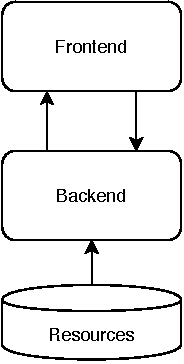
\includegraphics[scale=1]{figures/arch}
    \caption{Conceptual overview of the application}
    \label{fig:arch}
\end{figure}
\subsection{Architecture and Technologies}
For the architecture of the application, the common \textbf{Model-View-Controller} paradigm was used for a strict separation of functionality and an increased re-usability of the components as depicted in Figure \ref{fig:arch}.\par\medskip
The \textbf{Resources} represent the raw OpenStreetMap data which was provided in the \textit{Protocolbuffer Binary Format (PBF)}\footnote{\url{https://wiki.openstreetmap.org/wiki/PBF_Format}}.\par\medskip
The \textbf{Backend} provides the core functionality and implements algorithms on the OpenStreetMap data.
It is implemented as Web Server in \textit{Rust}\footnote{\url{https://www.rust-lang.org}}.
The core functionality of the Backend includes (i) a parser to map the OpenStreetMap data to a domain model representation in Rust,
(ii) a shortest path algorithm, and (iii) an \textit{Application Programming Interface} (API) to expose the functionality for access from the Frontend.\par\medskip
The \textbf{Frontend} is built using the \textit{React}\footnote{\url{https://reactjs.org}} Web Framework and \textit{Leaflet}\footnote{\url{https://leafletjs.com}}. Leaflet is an open-source JavaScript library for interactive maps based on OpenStreetMap.
Leaflet is used to provide a user-friendly map and allows to e.g. set markers or draw routes.
Figure \ref{fig:base_ui} displays the Frontend in its initial state.
The Frontend interacts with the Backend via \textit{HTTP} requests.
\begin{figure}[h]
    \centering
    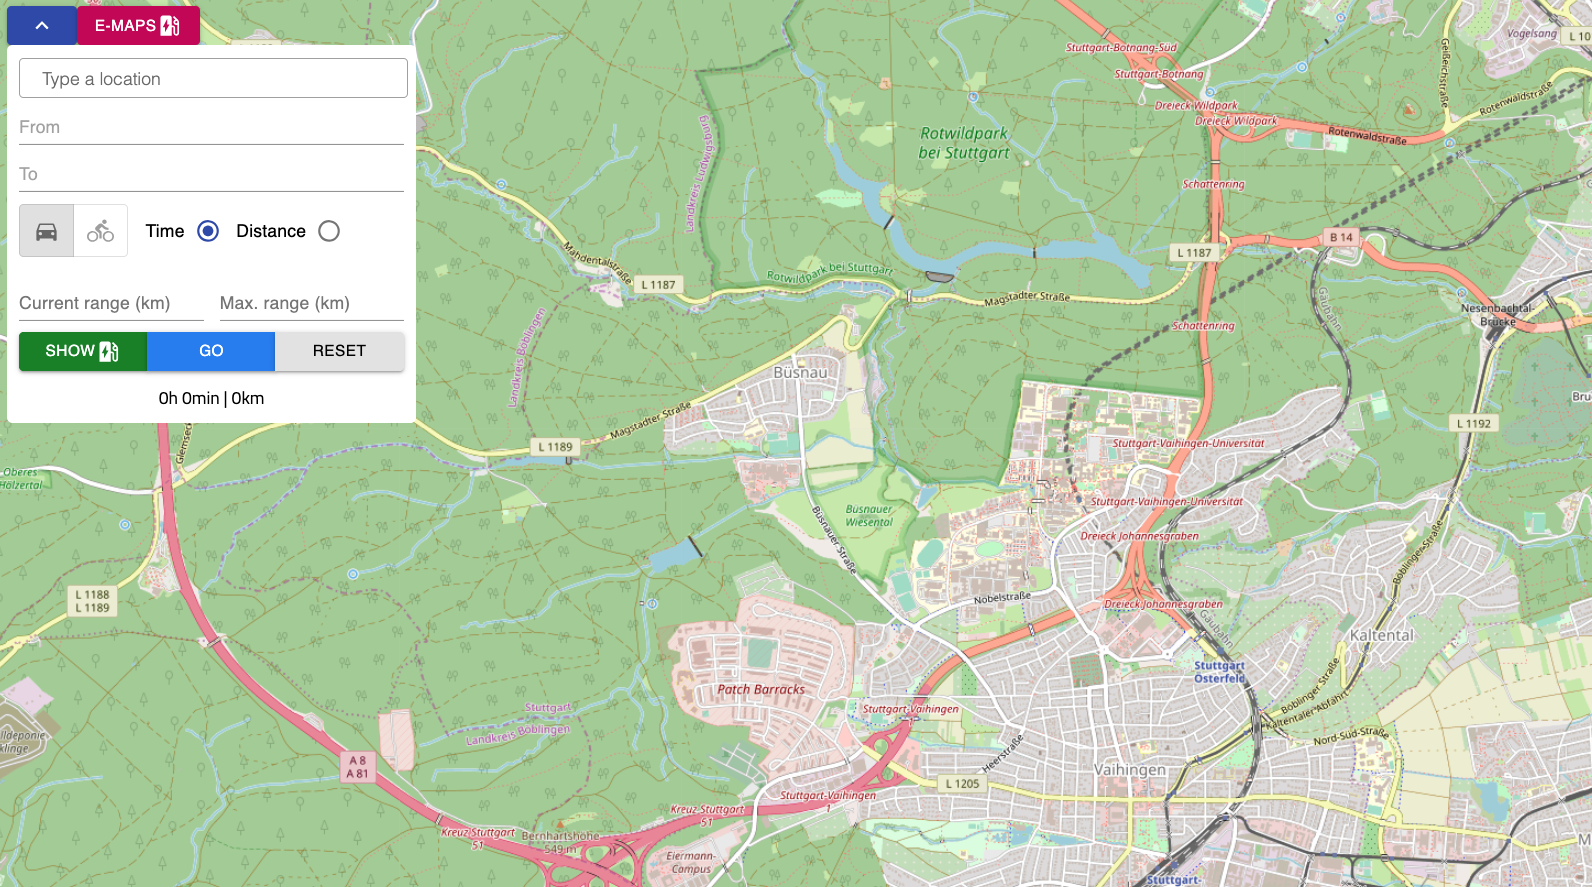
\includegraphics[scale=0.27]{figures/base_ui}
    \caption{Screenshot of the Frontend}
    \label{fig:base_ui}
\end{figure}
\subsection{Graph}
The Backend parses the graph data from OpenStreetMap in the PBF format.
Only necessary data is parsed from the PBF file for performance and efficiency reasons.
We focus on \textit{ways}, \textit{nodes}, and \textit{amenities} in OpenStreetMap. A node in OpenStreetMap is a single geographical data point with latitude and longitude. A way is a combination of multiple nodes building a sequence, e.g. a street.
Amenities are arbitrary geographical POIs, e.g. a restaurant, a bar, or a charging station.
Amenities are stored as Key-Value-Pairs in OpenStreetMap, e.g. $\lbrace amenity: charging\_station \rbrace$.
The implementation of this route planner focuses on electric cars and electric bikes, hence we only parse ways where cars and bikes are allowed to drive on.
Furthermore, we parse charging stations from the amenities to be able to consider those later on when calculating a route.\par\medskip
Our graph is structured as follows: $G = \lbrace N, E, O, C, CN \rbrace$ with (i) $N$ being a set of nodes, (ii) $E$ being a set of edges, (iii) $O$ being a offset array, (iv) $C$ being a cell hashmap and $CN$ being a set of nodes that represent a charging station.
The offset array is used to efficiently access the edges of a node. The cell hashmap is used to create a grid layer above the graph to speed up the search of the nearest node in the graph for given coordinates.
While creating the graph, every node is hashed into a grid cell using the predecimal digits of latitude and longitude of its coordinates.\par\smallskip
When the user requests a shortest path calculation from the Frontend, arbitrary start and goal locations may be passed. 
Since we only parsed ways that are valid for cars and bikes, the start and goal locations may not be present in our graph.
Thus, we may need to locate the nearest node in our graph to the start and goal location as passed by the user.\par\smallskip
Let us assume we want to locate the nearest node in our graph for a node called $n$.
First, we locate $n$ in the grid by using the predecimal digits of its coordinates. 
Then, we calculate the distance of all nodes in the cell to $n$ and choose the node with the smallest distance to $n$.
Since the nearest node to $n$ may be in another cell, we also check neighboring cells for the nearest neighbor.\par\medskip
To extract charging stations from OpenStreetMap, we check for each node if a Key-Value-Pair $\lbrace amenity: charging\_station \rbrace$ exists, i.e. if the node is tagged as charging station in OpenStreetMap.
Besides that, OpenStreetMap data may also provide information about the vehicles that can be charged at a charging station.
However, since OpenStreetMap is community-driven and based on user-generated data, not all charging stations contain information about the vehicles that can be charged.
Thus, for charging stations without further information, we just assume that both cars and bikes can be charged.
Hence, a charging station in our graph model contains coordinates, an enum indicating the vehicles that can be charged, and an identifier.
\subsection{Routing}
To route between two nodes in our graph, we use Dijkstra's Shortest Path Algorithm \cite{Dijkstra1959}.
The user is able to select between routing for shortest time or shortest distance, as visible in Figure \ref{fig:input}.
\subsection{Routing for Electric Vehicles}
The main functionality of this project is a route planner that considers the current and maximum range of electric vehicles, as well as the availability of charging stations to determine a route where an electric vehicle never runs out of battery.
\begin{figure}[h]
    \centering
    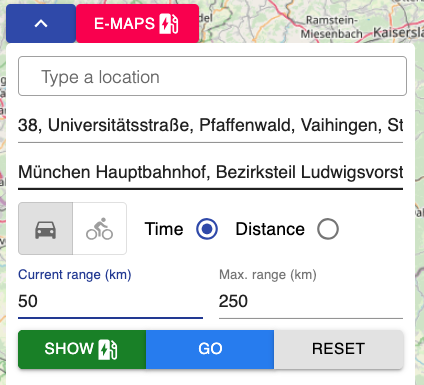
\includegraphics[scale=0.45]{figures/input}
    \caption{Modal for the user to e.g. enter current and maximum range}
    \label{fig:input}
\end{figure}
Figure \ref{fig:input} depicts the modal where the user can enter the current and maximum range of the electric vehicle used for travelling.
Once a start and goal location is chosen, the user can submit the request for route planning including the parameters of current and maximum range to the Backend.
The pseudo code depicted in Algorithm \ref{alg:route} simplifies the processing of the Backend once receiving such a request.\par\bigskip
\begin{algorithm}[H]
 \KwData{start coordinates, goal coordinates, current range, maximum range}
 \KwResult{route}
naive route $\leftarrow$  shortest path(start coordinates, goal coordinates)\;
required range $\leftarrow$ route.distance\;
 \While{required range > current range}{
 charging station coordinates $\leftarrow$ find optimal charging station coordinates\;
 route to charging $\leftarrow$ shortest path(start coordinates, charging station coordinates)\;
 route $\leftarrow$ route + route to charging\;
 
 current range $\leftarrow$ maximum range\;
 start coordinates $\leftarrow$ charging station coordinates\;
 
 route to goal $\leftarrow$ shortest path(start coordinates, goal coordinates)\;
 required range $\leftarrow$ route to goal.distance\;
 
  \If{required range < current range}{
    route $\leftarrow$ route + route to goal\;
     \Return{route}
   }
 }
 \Return{naive route}
 \caption{Simplified route calculation}
 \label{alg:route}
\end{algorithm}\par\bigskip
At first, we calculate the shortest path based on the start and goal parameters.
In line 3, we check if the distance of the shortest path surpasses our current range, i.e. if we need to charge our electric vehicle to travel from start to goal.
If the current range is sufficient for the calculated shortest path, we jump to line 16 and return the route to the Frontend.
If the current range is not sufficient, we need to visit at least one charging station.
Hence, we need to determine a charging station to visit, based on the start, goal, the current and maximum range, as well as our means of transportation (car or bike).\par\medskip
This calculation is depicted in Algorithm \ref{alg:charg}. 
After initializing variables we need later on, we start iterating over all charging stations of our graph in line 5.
In line 6, we check if the current charging station supports the means of transportation passed by the user.
If this is the case, we need to determine whether the current charging station is within our current range, i.e. if the range of our electric vehicle is sufficient to reach the charging station.
\par\bigskip
\begin{algorithm}[H]
	\KwData{start coordinates, goal coordinates, current range, transportation mode}
	\KwResult{chosen charging station}
	
	global min distance sum $\leftarrow$ max\;
	chosen charging station $\leftarrow$ null\;
	range utilization $\leftarrow$ 0.5\;
	haversine distance multiplier $\leftarrow$ 1.5\;
	\For{charging station \textbf{in} charging stations}{
		\If{charging station.supported \textbf{contains} transportation mode}{
			temp distance from start $\leftarrow$ distance(start coordinates, charging station)\;
			\If{temp distance from start $\times$ haversine distance multiplier =< current range}{
				\If{temp distance from start >= current range $\times$ range utilization treshold} {
					temp distance to goal $\leftarrow$ distance (goal coordinates, charging station)\;
					temp dist sum = temp distance from start + temp distance to goal\;
					\If{temp dist sum < global min distance sum}{
						global min distance sum $\leftarrow$ temp dist sum\;
						chosen charging station $\leftarrow$ charging station\;
					}
				}
			}
		}
	}
	\Return{chosen charging station}
	\caption{Simplified charging station coordinates calculation}
	\label{alg:charg}
\end{algorithm}\par\bigskip
To do this, we need to calculate the distance from the start to the current charging station.
Due to performance and efficiency, we do not calculate this distance via our shortest path algorithm, but with the haversine distance formula \cite{10.2307/2309088}, which determines the great-circle distance between two points on a sphere.
Since the distance for a shortest path between two points on a road network is bigger than the haversine distance, we need to make sure that the current charging station is actually reachable with our current range considering the actual distance of a shortest path on a road network.
\begin{figure}[h]
	\centering
	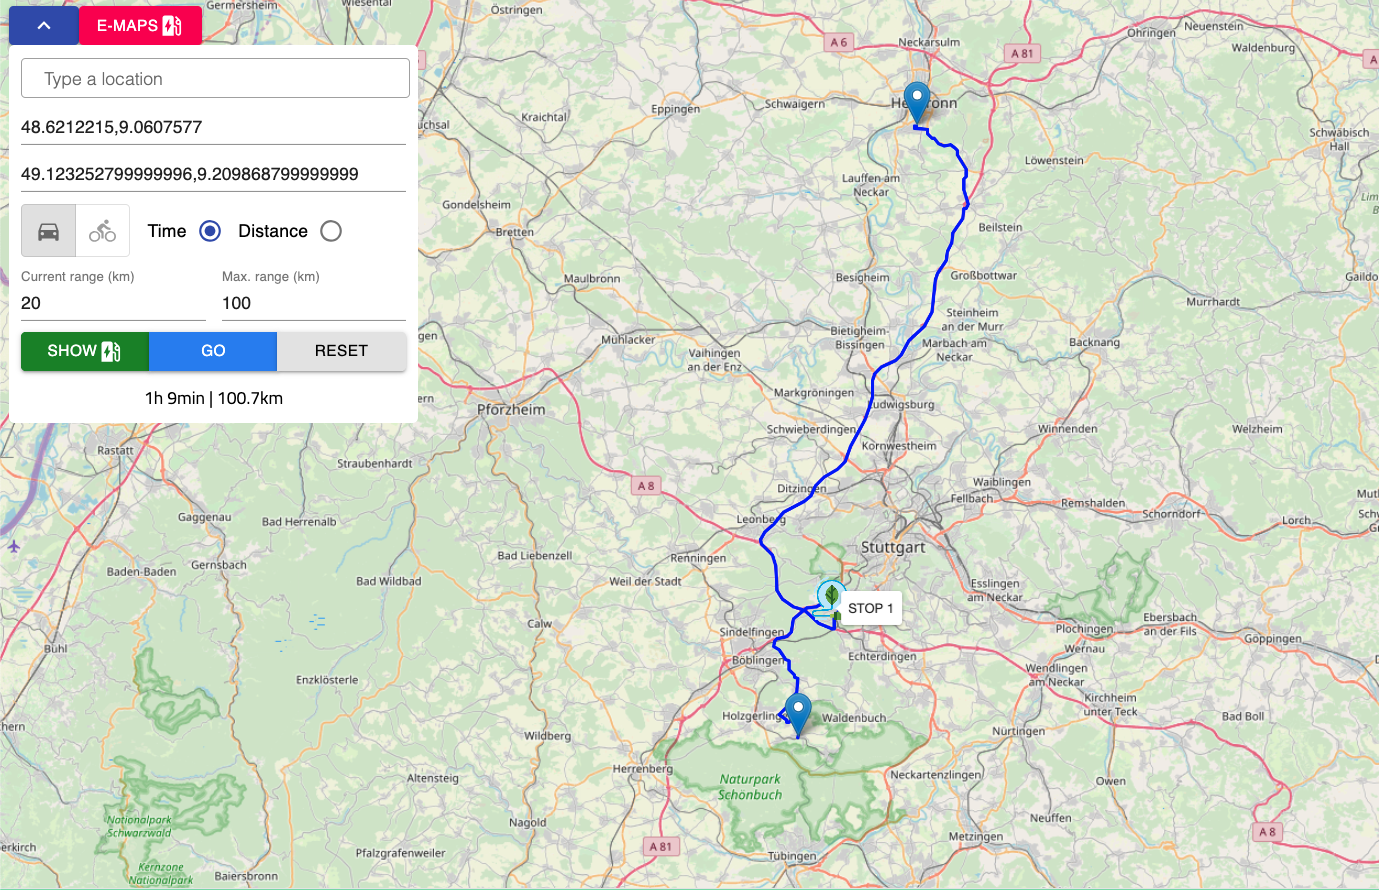
\includegraphics[scale=0.27]{figures/success}
	\caption{Successfully calculation of route with charging stations}
	\label{fig:success}
\end{figure}
\begin{figure}[h]
	\centering
	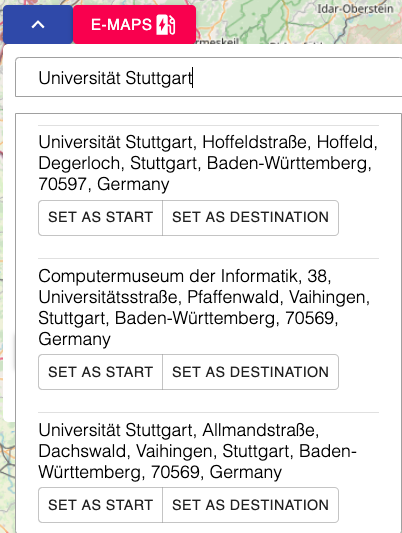
\includegraphics[scale=0.4]{figures/search}
	\caption{Search via Nominatim}
	\label{fig:search}
\end{figure}
\begin{figure}[h]
	\centering
	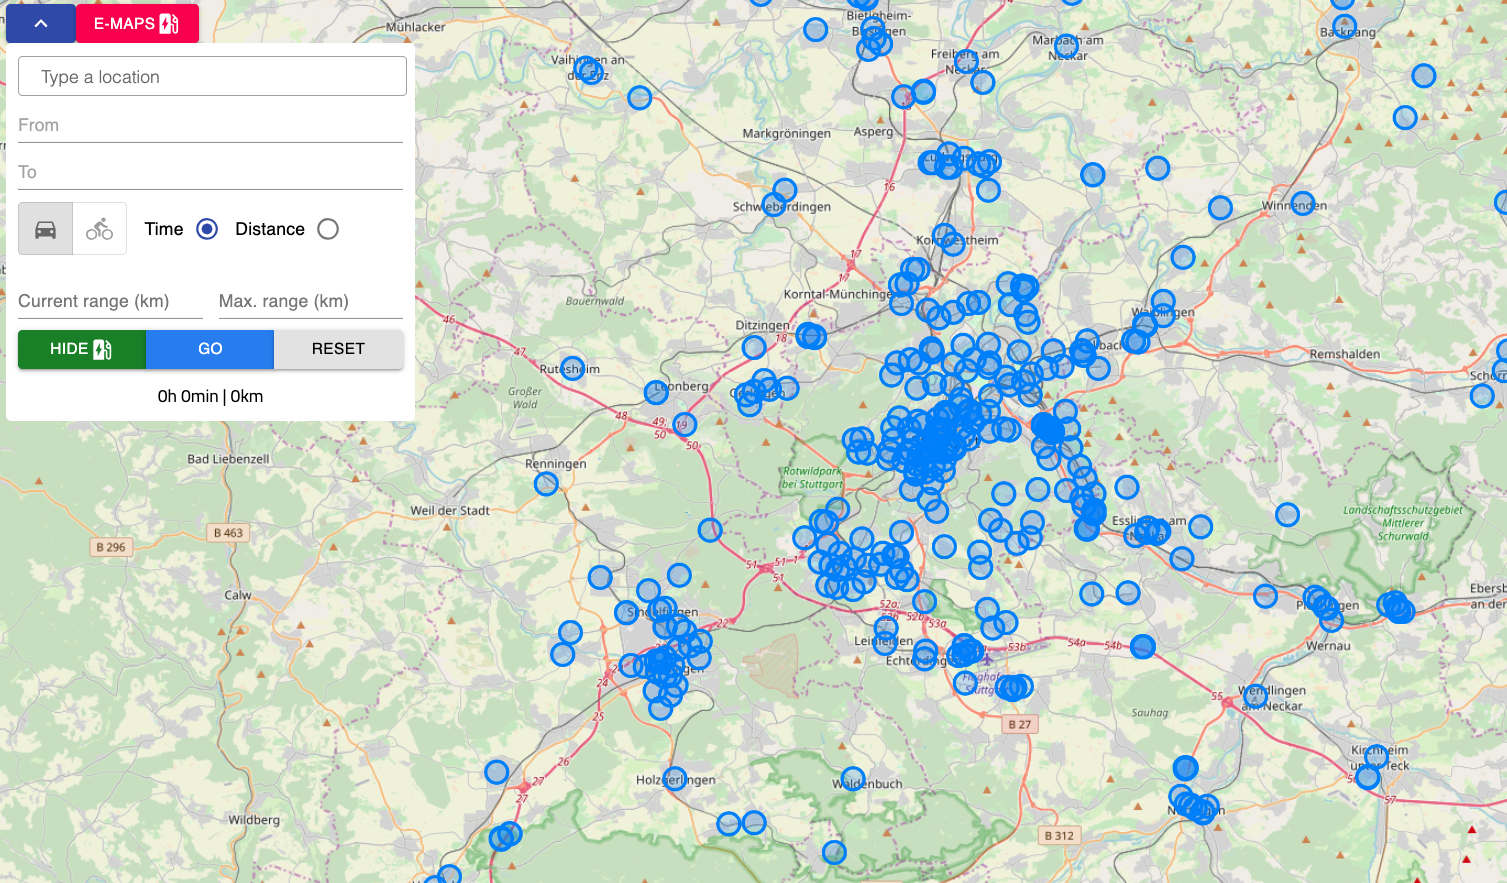
\includegraphics[scale=0.23]{figures/wide}
	\caption{Display all charging stations}
	\label{fig:charging}
\end{figure}
To ensure this, we use a multiplier of 1.5 as a heuristic for the haversine distance between the start and the charging station when comparing it to our current range as seen in line 8.
By using this value, we assume that the actual shortest path distance between two points on our road network is less or equal than $1.5$ times the haversine distance.
If the distance to the charging station is within our current range, we check in line 9 if at least 50\% of our current range is utilized to avoid wasting our range.
If at least 50\% of our range is utilized, we calculate the haversine distance from the current charging station to the goal.
In line 11, we sum up the haversine distances from the start to the current charging station, and from the charging station to the goal, as we want to determine the charging station with the smallest total distance between start, charging station and goal.
In line 12, we check if the sum is smaller than the current minimal total distance and, if this is the case, update the current global minimal distance sum and the chosen charging station accordingly.\par\medskip
Once we determined a charging station with Algorithm \ref{alg:charg}, we jump back to Algorithm \ref{alg:route} and calculate the shortest path from the start location to the chosen charging station location.
Then, we set our current range as maximum range, since we assume that we fully charged our electric vehicle, and replace the original start with the charging station as depicted in line 8 and 9.
Following, we calculate the shortest path from our new start to the goal location, and update the required range accordingly.
In line 11, we check if the required range is less or equal our current range, i.e. if the remaining distance does not require further charging, and if that is the case, we concatenate the calculated routes to one single route and return it in line 12 and 13.
However, if the remaining distance is still bigger than our current range, we jump back to the start of the while loop in line 4 and repeat the procedure until the remaining distance is within our current range.\par\bigskip
Figure \ref{fig:success} shows the Frontend with a successfully calculated route with charging stations.
The visited charging stations are highlighted for the user. \\
\subsection{Further Features}
Another feature of the application is the use of the \textit{Nominatim}\footnote{\url{https://nominatim.openstreetmap.org}} API to allow the user to search for places, cities or Point-Of-Interests (POIs) as seen in Figure \ref{fig:search}.
Furthermore, it is possible to show (or hide) all charging stations that exist, as seen in Figure \ref{fig:charging}.
These charging stations are, upon request, fetched from the backend via a HTTP GET request and rendered.
\section{Limitations and Related Work}
Since this project was within the scope of the lecture \textit{Fachpraktikum Algorithms on OpenStreetMap Data} the time spent on the concept and implementation was limited.
Hence, the route calculation with charging stations may not be optimal, especially determining the charging stations on the route.
Furthermore, considering the elevation profile of the road network might help to determine more energy efficient routes for electric vehicles, i.e. routes that go downhill or have a low elevation in general.\par\medskip
For example, Artmeier et al. \cite{Artmeier2010} proposed an extension to general shortest-path algorithms that address the problem of energy-optimal routing by extending a graph with a weight function representing the energy consumption \cite{Artmeier2010}.
To achieve a better routing for electric vehicles in terms of energy efficiency, a similar approach could be implemented on top of this project.\par\medskip
Worley et al. \cite{Worley2012} presented a model that addresses the problem of locating charging stations and calculate routes for electric vehicles based on discrete integer programming optimization and the traditional Vehicle Routing Problem \cite{Worley2012} that could be used to optimize the current implementation.
\section{Conclusion}
This project demonstrated the use and suitability of OpenStreetMap road network and amenity data to perform route planning for electric vehicles.
The implemented application is a route planner that considers the limited cruising range of electric vehicles, as well as the availability of charging stations along the route with the primary goal to avoid running out of power.
\bibliographystyle{alpha}
\bibliography{ref}
\end{document}
